\chapter{Background on Biological Collections}\label{biodiversity_data}

%\chapter{Understanding Biological Collections Data}\label{biodiversity_data}

% Biological collections
% Also known as natural museum or Natural History Collections (NHC).
% Biological collections such as herbaria and museums are a valuable source of biodiversity data.
% Many new species are discovered from collections samples \cite{Kemp2015}.
% Data collection is typically opportunistic.
% In scientific biological collections specimens are vouchered \cite{}.
% However, we still face the challenge of digitizing specimens in biological collections \cite{Hardisty2013}.


% The relevance of herbarium collections for conservation \cite{Nualart2017}


% Citizen Science projects
% Data from citizen science projects are structured similarly, with a few differences: (i) absence of vouchered specimens; (ii) taxonomic determinations result from a collaborative community, not necessarily composed of specialists. 




% Biological collections data coverage and completeness \cite{Funk1999}.
% Completeness: How much of data representing the real distribution of a species has actually been collected?
% \cite{Jacobs2017}
% Completeness of biodiversity databases \cite{Soberon2007}


% Describing and publishing digitized datasets
% Data description (metadata).
% Data publication (Darwin Core).

% Although information about the occurrence of specimen in regions is turning massive and freely available, users of such data must be aware of some inherent caveats, coming from how the context in which data was recorded. 
% Not all questions can be readily answered with such data, as there might be taxonomic, spatial,... biases.

%% As it is common practice for botanists to record each species once during field work, some important ecological attributes such as the species abundance are not to be directly inferred from such data. {check van Gemerden 2005, from Haripersaud2009}


% Biological collections are composed of aggregates of multiple biodiversity surveys, each recorded with particular methodologies
% Records sampled using distinct methodologies can be combined for optimizing data use \cite{VanGemerden2005}.

% Limitations in NHM data \cite{Graham2004 box3}
% Errors
% Biases
% Presence vc presence-absence data


% Sources of bias \cite{Daru2017, Haripersaud2009}
% Collector bias
% Trait bias
% Taxonomic bias
% Historical bias
% Seasonal bias
% Geographical bias




% ==========================
% ==========================
% Types of biodiversity data
% --------------------------

% Give an overview of commonly used types of biodiversity data
% Survey data (species checklists) -> examples: Catalogue of life
% Here we're interested in Species occurrence data

% ===============
% Occurrence data
% ---------------

% Characteristics of occurrence data?
%  Punctual data, often obtained in an opportunistic fashion
%  May include collectors field notes.
%  Main assets of a occurrence record: taxon, location, datetime {Graham2004} -> for us, also collectors

%% What are applications of occurrence data?
%%   - Species Distribution Modeling
%%   - Discovery of new species (check Kemp2015 - Museums: The endangered dead. )

%% Sources of occurrence data?
%%   - Biological collections / Museums;
%%   - Crowdsourcing/citizen science projects;

%% Limitations and caveats
%%   - Biases: collector bias, taxonomic bias, geographic bias...
%%   - {Graham2004 box3}
%%%% Kadmon, R., O. Farber, and A. Danin. 2004. Effect of roadside bias on the accuracy of predictive maps produced by bioclimatic models


% Collecting bias
% A mechanism for spatially characterizing collecting bias using Thiessen polygons \cite{Schulman2007}


%% Presence/absence data
%%   - {Graham2004 box3}


% ============
% Data quality
% ------------
% [Soberon2004]

% Data quality among collection records is uneven -> worse for large datasets and for datasets composed by multiple sources
% Procedures are needed for correcting problems

% Quality issues: 
%% Determination issues: many specimens are incorrectly identified;
%% outdated taxonomy;
%% georreferencing errors.

% Data atomicity issues:
% Some fields are not atomic: more than one entity is represented as a single data element. 
% In the recordedBy field, Darwin Core standards state that distinct names should be separated by | (delimiter).
% This varies depending on the standard a collection uses. For example, the BRAHMS system recommends using a ';' as the delimiter.
% BRAHMS docs: https://herbaria.plants.ox.ac.uk/bol/brahms/support/documentation

% Identity issues:
% Entities are not guaranteed to have the same ids through distinct datasets.
% Even in the same datasets there may be variations in their names
% this is specially problematic for fields like the collectors field, which is overlooked for most applications of such data. 
% Some standards provide guidelines for including collectors names: last name + first initials...
% However different standards give distinct guidelines and thus name variants are common.
% How to map all name variants to the same entity? -> This leads to the Entity-resolution problem

% Data fit for use

In order to make data fit for its intended use the analyst must perform data cleaning.

% =============
% Data cleaning
% -------------
%[Chapman2005a]

% Why do we need data cleaning? -> We must make data fit for its indended use

% Goal: improving data quality, removing or treating entries that are 

% Adopting standardized collectors names
% Checking collectors itineraries -> look for the spatial pattern of records by the collector


% ================
% References
% ----------------
%% Museum-based informatics{Graham2004}


\begin{figure}[h!]
  	\centering
    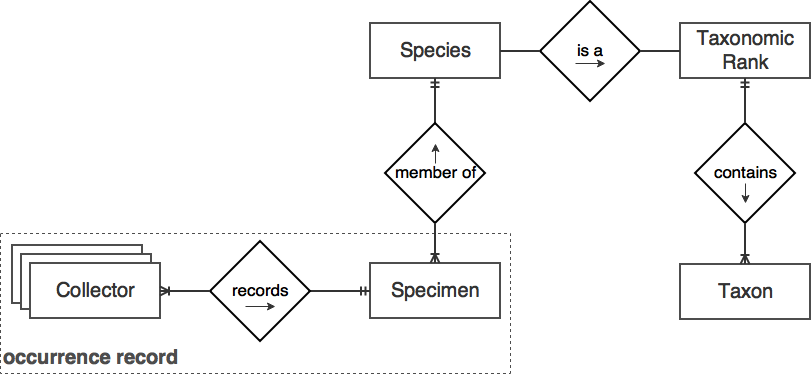
\includegraphics[width=0.8\linewidth]{figures/er_occurrence.png}
    \caption{Entity-relationship diagram for occurrences.}
    \label{fig:er_occurrences}
\end{figure}


% =====================
% Terms and Definitions
% ---------------------
Before delving into the characterization of biodiversity data we review the definitions of some domain-specific terms that will be used throughout this text. 
We specifically use definitions from the \textit{International Code of Nomenclature for algae, fungi and plants} (ICN) \cite{McNeill2012}. This document outlines a set of rules and guidelines for scientifically naming and grouping plants, fungi and algae, consisting of a universally adopted reference by the botanical scientific community. Nomenclature best-practices for other groups of organisms are governed by other (though similar) documents.

\paragraph*{Taxonomy}
Within the domain of biology taxonomy is, in a general sense, the science of classification of organisms. 
Organisms are classified in a hierarchical system, where more specific groupings of organisms are nested within broader ones. 
For an analogy with set theory, a taxonomic classification system can be thought as being similar to a hereditary (or pure) set, in that all members in a set are, recursively, also required to be sets. In our case, however, we allow the existence of non-set objects only in the lowest-level set, which is the most specific grouping of organisms a taxonomist can come up with.

\paragraph*{Taxonomic Rank.}
The taxonomic rank of a grouping of organisms is the level of the taxonomic hierarchy at which it is defined. The most relevant ranks adopted in botany (in descending hierarchical order) are \textit{Kingdom}, \textit{Phylum} (or \textit{Division}), \textit{Class}, \textit{Order}, \textit{Family}, \textit{Genus}, \textit{Species}, as stated in \textit{Art. $3.1$} of ICN.

\paragraph*{Species.}
Species is one of the taxonomic ranks organisms can be determined by professional taxonomists as belonging to. It is regarded to be a basic unit of taxonomic classification, although organisms can be further classified in lower-hierarchy taxonomic ranks (infraspecific ranks).
Differently from other ranks, the name of a species is composed using a binomial nomenclature system, in which the name of the genus it belongs to is appended to a \textit{specific epithet}.
Examples of species names are \textit{Caryocar brasiliense}, \textit{Myrcia guianensis}, \textit{Solanum lycocarpum}.

\paragraph*{Specimen.}
When botanists sample organisms in field they either collect part of the organism (\textit{e.g.} a branch of a tree), the entire organism (\textit{e.g.} the entire body of a weed) or multiple individuals of the same type (\textit{e.g.} a bunch of identical, very small-sized mosses). 
Any of these collected biological materials is an evidence of the existence of a particular organism at some place and time, and should be properly deposited in a biological collection. A specimen is defined as one of such evidences, and refers to a punctual observation of a single kind of organism. For the formal definition refer to \textit{Art. $8.2$} of ICN. 
Although a specimen could be classified by a taxonomist as being a representative of a given species, this is not a requirement for it to be included in scientific collections. Although taxonomists classify specimens in a best effort manner (the most taxonomically precise as possible), sometimes only higher ranks can be determined. The highest taxonomic rank at which the specimen could be identified is known as its \textbf{taxonomic resolution}.
After properly deposited in a biological collection, each record receives a taxonomic identification that assigns the individual to a taxonomic group (a taxon), in a best-effort manner.

\paragraph*{Taxon.}

A taxon is a taxonomic group of organisms at the level of any rank (ICN \textit{Art.1.1}). Notice that the plural is \textbf{taxa}.




% Data Quality

% Preparing data 
% Data Selection
% Data Cleaning


% The Entity Resolution problem
\cite{Bhattacharya2007}
